\documentclass[A4,12pt, utf8]{article}
\usepackage{tikz}
\usepackage[
    backend=biber,
    style=authoryear-icomp,
    sortlocale=de_DE,
    natbib=true,
    url=false, 
    doi=true,
    eprint=false
]{biblatex}
\usepackage{listings}
\usepackage{xcolor}
\usepackage{hyperref}
\usepackage{pgf}
\usepackage{tikz}
\usetikzlibrary{arrows,automata}
\usepackage{todonotes}
\usepackage{dirtree}
\usepackage{pdflscape}
\usepackage{csquotes}
\MakeOuterQuote{"}


\newcommand{\tinytodo}[2][]
   {\todo[caption={#2}, size=\small, #1]{\renewcommand{\baselinestretch}{0.5}\selectfont#2\par}}

\colorlet{punct}{red!60!black}
\definecolor{background}{HTML}{EEEEEE}
\definecolor{delim}{RGB}{20,105,176}
\colorlet{numb}{magenta!60!black}

\lstdefinelanguage{json}{
    basicstyle=\normalfont\ttfamily,
    % numbers=left,
    % numberstyle=\scriptsize,
    % stepnumber=1,
    % numbersep=8pt,
    showstringspaces=false,
    breaklines=true,
    frame=lines,
    backgroundcolor=\color{background},
    literate=
     *{0}{{{\color{numb}0}}}{1}
      {1}{{{\color{numb}1}}}{1}
      {2}{{{\color{numb}2}}}{1}
      {3}{{{\color{numb}3}}}{1}
      {4}{{{\color{numb}4}}}{1}
      {5}{{{\color{numb}5}}}{1}
      {6}{{{\color{numb}6}}}{1}
      {7}{{{\color{numb}7}}}{1}
      {8}{{{\color{numb}8}}}{1}
      {9}{{{\color{numb}9}}}{1}
      {:}{{{\color{punct}{:}}}}{1}
      {,}{{{\color{punct}{,}}}}{1}
      {\{}{{{\color{delim}{\{}}}}{1}
      {\}}{{{\color{delim}{\}}}}}{1}
      {[}{{{\color{delim}{[}}}}{1}
      {]}{{{\color{delim}{]}}}}{1},
}
% \addbibresource{linked.bib}

\newcounter{treeline}

\newcommand{\treeroot}[1]{% Title
\node[above] at (0,0) {#1};%
\setcounter{treeline}{0}
}

\newcommand{\treeentry}[2]{% Title, Level
\draw[->] (#2-1,-\value{treeline}/2) -- (#2-1,-\value{treeline}/2-0.5) -- (#2+0.5,-\value{treeline}/2-0.5) node[right] {#1};
\stepcounter{treeline}
}

\newcommand{\altentry}[2]{% Title, Level
\draw[->] (#2-1,-\value{treeline}/2) -- (#2-1,-\value{treeline}/2-0.5) -- (#2+0.5,-\value{treeline}/2-0.5) node[right] {#1};
\foreach \x in {1,...,#2}
{   \draw (\x-1,-\value{treeline}/2) -- (\x-1,-\value{treeline}/2-0.5);
}
\stepcounter{treeline}
}


\title{emuLVC - Stucture of the angularjs app}
\author{Raphael Winkelmann}
\date{\today}
\begin{document}
  % \maketitle

\section{Schematic DB file structure on disc}

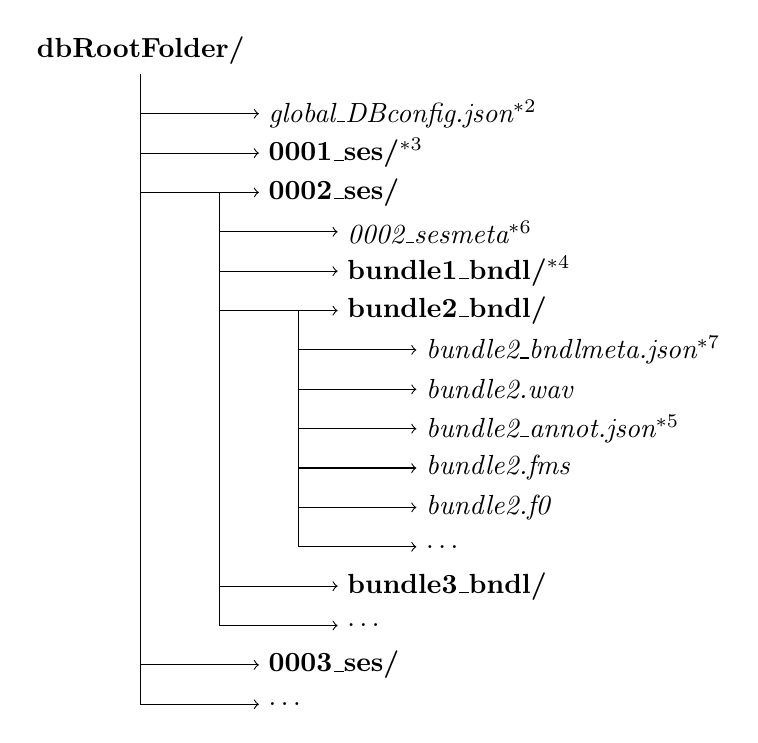
\begin{tikzpicture}
\treeroot{\textbf{dbRootFolder/}}
\altentry{\textit{global\_DBconfig.json$^{*2}$}}{1}
\altentry{\textbf{0001\_ses/$^{*3}$}}{1}
\altentry{\textbf{0002\_ses/}}{1}
\altentry{\textit{0002\_sesmeta$^{*6}$}}{2}
\altentry{\textbf{bundle1\_bndl/$^{*4}$}}{2}
\altentry{\textbf{bundle2\_bndl/}}{2}
\altentry{\textit{bundle2\_bndlmeta.json$^{*7}$}}{3}
\altentry{\textit{bundle2.wav}}{3}
\altentry{\textit{bundle2\_annot.json$^{*5}$}}{3}
\altentry{\textit{bundle2.fms}}{3}
\altentry{\textit{bundle2.f0}}{3}
\altentry{\dots}{3}
\altentry{\textbf{bundle3\_bndl/}}{2}
\altentry{\dots}{2}
\altentry{\textbf{0003\_ses/}}{1}
\altentry{\dots}{1}
\end{tikzpicture}


\begin{itemize}
  \item $^{*2}$: global config information file (similar to \textit{.tpl} file of old EMU). Specifies things like structure of hierarchy and possible perspectives to look at the DB (relevant for layout of labeler). \textit{\_DBconfig.json} is a fix suffix and the prefix should be the same as the database name field in the file itself.
  \item $^{*3}$: \textit{\_ses} is a fix suffix specifying the folder as being a session folder. Preceding this suffix can be anything as long it is unique on a session level (OS won't let you name two folders the same anyway...). If no session is required a dummy session is used called 0000\_ses.
  \item $^{*4}$: a bundle encapsulates what used to be known as an utterance in a folder. This includes signal files (\textit{wav, SSFF}) and the new annotation file (see $^{*5}$). Unknown file extensions are ignored. \textit{\_bndl} is a fix suffix specifying the folder as being a bundle folder.
  \item $^{*5}$: annotation file containing label and level information as well as hierarchical information (see listing 1). \textit{\_annot.json} is a fix suffix and the prefix should be the same as the bundle name.
  \item $^{*6}$: Optional session meta information file. Simple key-value json of the form \{"key1":"value1", "key2":"value2"\}
  \item $^{*7}$: Optional bundle meta information file. Simple key-value json of the form \{"key1":"value1", "key2":"value2"\}
\end{itemize}



%%%%%%%%%%%%%%%%%%%%%%%%%%%%%%%%%%%%%%
%%%%%%%%%%%%%%%%%%%%%%%%%%%%%%%%%%%%%%
%%%%%%%%%%%%%%%%%%%%%%%%%%%%%%%%%%%%%%
\section{File structure of json files}

The EMU-webApp supports several JSON file types for which individual schema are available (all of type:
\texttt{http://json-schema.org/draft-04/schema\#})

\section{Schema files}

There are two sets of schema files. The ones being used by the current live version of the web application 
(\url{http://ips-lmu.github.io/EMU-webApp/}) and the ones used by the current development version.
The two sets are usually quite similar if not identical as we try to keep the file definitions as
constant as possible.

The schema files used by the current live version are:

\todo[inline]{redo after schema cleanup}

\begin{itemize}
  \item \textbf{DBconfigFileSchema}: \href{https://github.com/IPS-LMU/EMU-webApp/blob/master/dist/schemaFiles/DBconfigFileSchema.json}{GitHub link}
  \item \textbf{annotationFileSchema}: \href{https://github.com/IPS-LMU/EMU-webApp/blob/master/dist/schemaFiles/annotationFileSchema.json}{GitHub link}
  \item \textbf{bundleSchema}: \href{https://github.com/IPS-LMU/EMU-webApp/blob/master/dist/schemaFiles/bundleSchema.json}{GitHub link}
  \item \textbf{bundleListSchema}: \href{https://github.com/IPS-LMU/EMU-webApp/blob/master/dist/schemaFiles/bundleListSchema.json}{GitHub link}
  \item \textbf{emuwebappConfigSchema}: \href{https://github.com/IPS-LMU/EMU-webApp/blob/master/dist/schemaFiles/emuwebappConfigSchema.json}{GitHub link}
  \item \textbf{emuwebappConfigSchema}: \href{https://github.com/IPS-LMU/EMU-webApp/blob/master/dist/schemaFiles/emuwebappConfigSchema.json}{GitHub link}
\end{itemize}

The schema files for the development version are:

\begin{itemize}
  \item \textbf{DBconfigFileSchema}: \href{https://github.com/IPS-LMU/EMU-webApp/blob/master/dist/schemaFiles/DBconfigFileSchema.json}{GitHub link}
  \item \textbf{annotationFileSchema}: \href{https://github.com/IPS-LMU/EMU-webApp/blob/master/dist/schemaFiles/annotationFileSchema.json}{GitHub link}
  \item \textbf{bundleSchema}: \href{https://github.com/IPS-LMU/EMU-webApp/blob/master/dist/schemaFiles/bundleSchema.json}{GitHub link}
  \item \textbf{bundleListSchema}: \href{https://github.com/IPS-LMU/EMU-webApp/blob/master/dist/schemaFiles/bundleListSchema.json}{GitHub link}
  \item \textbf{emuwebappConfigSchema}: \href{https://github.com/IPS-LMU/EMU-webApp/blob/master/dist/schemaFiles/emuwebappConfigSchema.json}{GitHub link}
  \item \textbf{emuwebappConfigSchema}: \href{https://github.com/IPS-LMU/EMU-webApp/blob/master/dist/schemaFiles/emuwebappConfigSchema.json}{GitHub link}
\end{itemize}


Examples of files that validate against these schemas can be found here: 

\todo[inline]{List files that validate here}


\begin{lstlisting}[caption=EMU-webApp internal derived signal representation, label=idsr, language=json,firstnumber=1]
{
  "filepath": "/path/to/msajc003.fms",
  "sampleRate" = 200,
  "origFreq" = 20000,
  "startTime" = 0.0025,
  "columns" = [
  {"name": "fm",
    "length": 4,
    "ssffDataType": "SHORT"
    "values" : [[0, 1042, 2072, 3170],
                [0, 1260, 2122, 3118],
                [0, 1339, 2293, 3258],
                ...]},
  {"name": "bw",
    "length": 4,
    "ssffDataType": "SHORT"
    "values" : [[0, 886, 371, 890],
                [0, 724, 567, 826],
                [0, 410, 664, 740],
                ...]}
  ]
}
\end{lstlisting}

\clearpage

%%%%%%%%%%%%%%%%%%%%%%
%%%%%%%%%%%%%%%%%%%%%%
%%%%%%%%%%%%%%%%%%%%%%
\section{Websocket protocol definition (Version 0.0.2)}

All notation in nodejs / javascript syntax. The \texttt{request.callbackID} variable is a UUID that is echoed by the server on every request to remap the response to the request on the client. \texttt{xxxxxxxx-xxxx-4xxx-yxxx-xxxxxxxxxxxx} is used as a placeholder for all UUIDs.

%%%%%%%%%%%%%%%%%%%%%%%%%%%%%
%%%%%%%%%%%%%%%%%%%%%%%%%%%%%
\subsection{Version history}
\begin{itemize}
  \item \textbf{0.0.1}: Initial protocol version
  \item \textbf{0.0.2}: Updated \texttt{\_bundle.json} schema (\texttt{ssffTrackName} $\rightarrow$ \texttt{fileExtention}) to remove SSFF file redundancy (current version)
  \item \textbf{0.0.3}: Future version to include EDITDBCONFIG operations (currently under development)
\end{itemize}


A graph depicting the protocol can be seen in figure \ref{fig:emuwsprot}

\begin{figure}[!ht]
\caption{EMU-webApp-websocket-protocol version 0.0.3 (currently under development) ($^{*1}$: has multiple subcommands! See section)}\label{fig:emuwsprot}
\begin{center}

\documentclass[tikz, convert={outfile=\jobname.svg}]{standalone}
\usetikzlibrary{shapes,arrows, backgrounds}
\begin{document}
\definecolor{emublue}{RGB}{13, 197, 255}
\definecolor{emulightgray}{RGB}{231, 231, 231}
% Define block styles

\tikzstyle{cmd} = [rectangle, draw, fill=emulightgray,
    text centered, rounded corners, font=\small]
\tikzstyle{states} = [draw, ellipse,fill=yellow, font=\small]

\begin{tikzpicture}[node distance = 1.3cm, auto, show background rectangle,
  background rectangle/.style={fill=white, opacity=0},
  color=black,
  help lines/.style={color=lightgray,line width=.2pt}]
    % Place nodes
    \node [states] (connect) {\texttt{disconnected state}};
    \node [cmd, below of=connect] (GETPROTOCOL) {\texttt{GETPROTOCOL}};
    \node [cmd, below of=GETPROTOCOL] (GETDOUSERMANAGEMENT) {\texttt{GETDOUSERMANAGEMENT}};
    \node [cmd, below of=GETDOUSERMANAGEMENT] (GETGLOBALDBCONFIG) {\texttt{GETGLOBALDBCONFIG}};
    \node [cmd, left of=GETDOUSERMANAGEMENT, node distance = 4cm] (LOGONUSER) {\texttt{LOGONUSER}};
    \node [cmd, below of=GETGLOBALDBCONFIG] (GETBUNDLELIST) {\texttt{GETBUNDLELIST}};

    \node [states, below of=GETBUNDLELIST] (connected) {\texttt{connected state}};

    \node [right of=connected, node distance = 4cm] (dummyBundleNode) {};
    \node [cmd, above of=dummyBundleNode] (GETBUNDLE) {\texttt{GETBUNDLE}};
    \node [cmd, below of=dummyBundleNode] (SAVEBUNDLE) {\texttt{SAVEBUNDLE}};

    \node [cmd, above of=GETBUNDLE] (DISCONNECTWARNING) {\texttt{DISCONNECTWARNING}};

    % \node [cmd, below of=connected, node distance = 2cm] (GETDOEDITDBCONFIG) {\texttt{GETDOEDITDBCONFIG}};
    % \node [cmd, left of=GETDOEDITDBCONFIG, node distance = 4cm] (EDITDBCONFIG) {\texttt{EDITDBCONFIG$^{*1}$}};

    % Draw edges
    \draw [->] (connect) -- (GETPROTOCOL);
    \draw [->] (GETPROTOCOL) -- (GETDOUSERMANAGEMENT);
    \draw [->] (GETDOUSERMANAGEMENT) -- node {no} (GETGLOBALDBCONFIG);
    \draw [->] (GETDOUSERMANAGEMENT) -- node {yes} (LOGONUSER);
    \draw [->] (LOGONUSER) |-  (GETGLOBALDBCONFIG);
    \draw [->] (GETGLOBALDBCONFIG) -- (GETBUNDLELIST);
    \draw [->] (GETBUNDLELIST) -- (connected);
    \draw [->] (connected) -- (DISCONNECTWARNING);
    \draw [->] (DISCONNECTWARNING) to [bend right=25] (connect);
    \draw [<->] (connected) -- (GETBUNDLE);
    \draw [<->] (connected) -- (SAVEBUNDLE);
    % \draw [->] (connected) -- (GETDOEDITDBCONFIG);
    % \draw [->] (GETDOEDITDBCONFIG) -- node {yes} (EDITDBCONFIG);
    % \draw [->] (EDITDBCONFIG) |-  (connected);
    % \draw [->] (GETDOEDITDBCONFIG.west) to [bend left=45] node {no}  (connected);

\end{tikzpicture}
\end{document}

\end{center}
\end{figure}

%%%%%%%%%%%%%%%%%%%%%%
%%%%%%%%%%%%%%%%%%%%%%
\subsection{The Protocol}

%%%%%%%%%%%%%%%%%%%%%%
\subsubsection{\texttt{GETPROTOCOL}}
\begin{center}
  \line(1,0){250}

  \textit{Initial request to see if client and server speak the same protocol.}

  \line(1,0){250}
\end{center}


\begin{lstlisting}[caption=Request content, language=json]
{
  'type': 'GETPROTOCOL', 
  'callbackID': 'xxxxxxxx-xxxx-4xxx-yxxx-xxxxxxxxxxxx'
}
\end{lstlisting}

\begin{lstlisting}[caption=response content, language=json]
{
  'callbackID': request.callbackID,
  'data': {
    'protocol': 'EMU-webApp-websocket-protocol',
    'version': '0.0.1'
  },
  'status': {
    'type': 'SUCCESS',
    'message': ''
  }
}
\end{lstlisting}

%%%%%%%%%%%%%%%%%%%%%%
\subsubsection{\texttt{GETDOUSERMANAGEMENT}}
\begin{center}
  \line(1,0){250}

  \textit{Ask server if a it wishes to perform user management (will toggle login dialog if YES)}

  \line(1,0){250}
\end{center}


\begin{lstlisting}[caption=Request content, language=json]
{
  'type': 'GETDOUSERMANAGEMENT', 
  'callbackID': 'xxxxxxxx-xxxx-4xxx-yxxx-xxxxxxxxxxxx'
}
\end{lstlisting}

\begin{lstlisting}[caption=response content, language=json]
{
  'callbackID': request.callbackID,
  'data': 'NO'
  'status': {
    'type': 'SUCCESS',
    'message': ''
  }
}
\end{lstlisting}

%%%%%%%%%%%%%%%%%%%%%%
\subsubsection{\texttt{LOGONUSER}}
\begin{center}
  \line(1,0){250}

  \textit{Ask server to log on user. Username and password are sent to server.}

  \line(1,0){250}
\end{center}

\begin{lstlisting}[caption=Request content, language=json]
{
  'type': 'LOGONUSER',
  'data': {
    'userName': 'smith', 
    'pwd':'mySecretPwd'
  },
  'callbackID': 'xxxxxxxx-xxxx-4xxx-yxxx-xxxxxxxxxxxx'
}
\end{lstlisting}

\begin{lstlisting}[caption=response content, language=json]
{
  'callbackID': request.callbackID,
  'data': 'BADUSERNAME' | 'BADPASSWORD' | 'LOGGEDON'
  'status': {
    'type': 'SUCCESS',
    'message': ''
  }
}
\end{lstlisting}

%%%%%%%%%%%%%%%%%%%%%%
\subsubsection{\texttt{GETGLOBALDBCONFIG}}
\begin{center}
  \line(1,0){250}

  \textit{Next the globalDBconfig.json is requested from the DB. This is needed for the level definitions (future version) $+$ the legal values of each level $+$ the custom config specified in the field EMU-webAppConfig}

  \line(1,0){250}
\end{center}


\begin{lstlisting}[caption=Request content, language=json]
{
  'type': 'GETGLOBALDBCONFIG', 
  'callbackID': 'xxxxxxxx-xxxx-4xxx-yxxx-xxxxxxxxxxxx'
}
\end{lstlisting}

\begin{lstlisting}[caption=response content, language=json]
{
  'callbackID': request.callbackID,
  'data': configData,
  'status': {
    'type': 'SUCCESS',
    'message': ''
  }
}
\end{lstlisting}
Where \texttt{configData} is the javascript object representing \texttt{globalDBconfig.json}

%%%%%%%%%%%%%%%%%%%%%%
\subsubsection{\texttt{GETBUNDLELIST}}
\begin{center}
  \line(1,0){250}

  \textit{Next a bundlelist is requested.}

  \line(1,0){250}
\end{center}


\begin{lstlisting}[caption=Request content, language=json]
{
  'type': 'GETBUNDLELIST', 
  'callbackID': 'xxxxxxxx-xxxx-4xxx-yxxx-xxxxxxxxxxxx'
}
\end{lstlisting}

\begin{lstlisting}[caption=response content, language=json]
{
  'callbackID': request.callbackID,
  'data': bundleList,
  'status': {
    'type': 'SUCCESS',
    'message': ''
  }
}
\end{lstlisting}

%%%%%%%%%%%%%%%%%%%%%%
\subsubsection{\texttt{GETBUNDLE}}
\begin{center}
  \line(1,0){250}

  \textit{After receiving the bundleList by default the first bundle in the bundleList is requested. This request is also sent when the user clicks a bundle in the bundleList}

  \line(1,0){250}
\end{center}


\begin{lstlisting}[caption=Request content, language=json]
{
  'type': 'GETBUNDLE',
  'name': 'msajc003',
  'session': '0000',
  'callbackID': 'xxxxxxxx-xxxx-4xxx-yxxx-xxxxxxxxxxxx'
}
\end{lstlisting}

\begin{lstlisting}[caption=response content, language=json]
{
  'callbackID': request.callbackID,
  'data': bundleData,
  'status': {
    'type': 'SUCCESS',
    'message': ''
  }
}
\end{lstlisting}
Where \texttt{bundleData} is the javascript object containing all the values of ssffTracks + audio + annotation.json in the DB (see example bundle for details).

%%%%%%%%%%%%%%%%%%%%%%
\subsubsection{\texttt{SAVEBUNDLE}}
\begin{center}
  \line(1,0){250}

  \textit{Function to be called if the user saves a loaded bundle (by pushing the save button).}

  \line(1,0){250}
\end{center}


\begin{lstlisting}[caption=Request content, language=json]
{
  'type': 'SAVEBUNDLE',
  'data': bundleData,
  'callbackID': 'xxxxxxxx-xxxx-4xxx-yxxx-xxxxxxxxxxxx'
}
\end{lstlisting}
Where \texttt{bundleData} is the javascript object OPTIONALLY containing the values of ssffTracks + audio + annotation.json in the DB (see example bundle for details). It only sends the data that has been altered.

\begin{lstlisting}[caption=response content, language=json]
{
  'callbackID': request.callbackID,
  'status': {
    'type': 'SUCCESS',
    'message': ''
  }
}
\end{lstlisting}

%%%%%%%%%%%%%%%%%%%%%%
\subsubsection{\texttt{GETDOEDITDBCONFIG}}
\label{GETDOEDITDBCONFIG}
\begin{center}
  \line(1,0){250}

  \textit{Ask server if it allows editing of the \_DBconfig}

  \line(1,0){250}
\end{center}


\begin{lstlisting}[caption=Request content, language=json]
{
  'type': 'GETDOEDITDBCONFIG', 
  'callbackID': 'xxxxxxxx-xxxx-4xxx-yxxx-xxxxxxxxxxxx'
}
\end{lstlisting}

\begin{lstlisting}[caption=response content, language=json]
{
  'callbackID': request.callbackID,
  'data': 'YES'
  'status': {
    'type': 'SUCCESS',
    'message': ''
  }
}
\end{lstlisting}


%%%%%%%%%%%%%%%%%%%%%%
\subsubsection{\texttt{EDITDBCONFIG}}
\label{EDITDBCONFIG}
\begin{center}
  \line(1,0){250}

  \textit{Send DBconfig edit command to server. Compared to the other protocol 
  request this request has several subtypes that specify the various edit operations
  to the \_DBconfig }

  \line(1,0){250}
\end{center}


\begin{lstlisting}[caption=Request content, language=json]
{
  'type': 'EDITDBCONFIG',
  'subtype': 'ADDLEVELDEFINITION', 
  'data': newLevelDefinition
  'callbackID': 'xxxxxxxx-xxxx-4xxx-yxxx-xxxxxxxxxxxx'
}
\end{lstlisting}

\begin{lstlisting}[caption=response content (if changes could be applied to DB), language=json]
{
  'callbackID': request.callbackID,
  'data': 'YES'
  'status': {
    'type': 'SUCCESS',
    'message': ''
  }
}
\end{lstlisting}

\begin{lstlisting}[caption=response content (if changes could NOT be applied to DB), language=json]
{
  'callbackID': request.callbackID,
  'data': {
    'EDITDBCONFIG-errorMsg': '',
    'subtype': 'MODIFYATTRIBUTEDEFINITION',
    'levelDefinitionsName': 'Phonetic',
    'attributeDefinitionsName': 'IPA'
  },
  'status': {
    'type': 'SUCCESS',
    'message': ''
  }
}
\end{lstlisting}


The current subtypes are: 

\begin{itemize}
  \item \texttt{ADDLEVELDEFINITION}
  \item \texttt{ADDATTRIBUTEDEFINITION}
  \item \texttt{MODIFYATTRIBUTEDEFINITION}
\end{itemize}

%%%%%%%%%%%%%%%%%%%%%%
\subsubsection{\texttt{DISCONNECTWARNING}}
\begin{center}
  \line(1,0){250}

  \textit{Function that tells server that it is about to disconnect. This is currently needed because the httpuv R package can't listen to the websockets own close event.}

  \line(1,0){250}
\end{center}


\begin{lstlisting}[caption=Request content, language=json]
{
  'type': 'DISCONNECTWARNING'
  'callbackID': 'xxxxxxxx-xxxx-4xxx-yxxx-xxxxxxxxxxxx'
}
\end{lstlisting}

\begin{lstlisting}[caption=response content, language=json]
{
  'callbackID': request.callbackID,
  'status': {
    'type': 'SUCCESS',
    'message': ''
  }
}
\end{lstlisting}



%%%%%%%%%%%%%%%%%%%%%%
\subsection{Error handling}

If an error occurs with any of the request types above a response should still be sent to the client. The status of this response should be set to \texttt{ERROR} and an error message should be given in the message field. This message will then be displayed on the client.

\begin{lstlisting}[caption=ERROR response content, language=json]
{
  'callbackID': request.callbackID,
  'status': {
    'type': 'ERROR',
    'message': 'An error occured trying to read a file from disk. Please make sure: /path/to/file exists or check the config...
  }
}
\end{lstlisting}


\end{document}